% Provenance (never printed): 6e geography and cycle 3 sciences (locating a
% place on the globe: parallels, meridians, latitude, longitude; the Earth's
% rotation and time zones); see sources/book1/PROVENANCE.md.
% Book 1, grade 6, chapter 2.
\chapter{Latitude, Longitude and Time Zones}\label{ch:g6:latitude-longitude}

Night has fallen on the \omterm{def:g2:water-on-earth:ocean}{ocean}. On the deck of a sailing ship, in the year
1750, the navigator lifts his instrument towards a bright star and measures
how high it stands above the \omterm{def:g2:water-on-earth:ocean}{sea}. A few minutes of work, and he knows how
far north of the \omterm{def:g3:continents-and-oceans:equator}{equator} the ship is. But how far east or west? That, he
cannot tell. The problem was so serious that in 1714 the British parliament
had promised a large prize to whoever found a way to measure it at \omterm{def:g2:water-on-earth:ocean}{sea}.
Today, the phone in your pocket gives both answers in one second.
% ledger: rmg:15deg-per-hour, rmg:longitude-act-1714

\begin{omfigure}
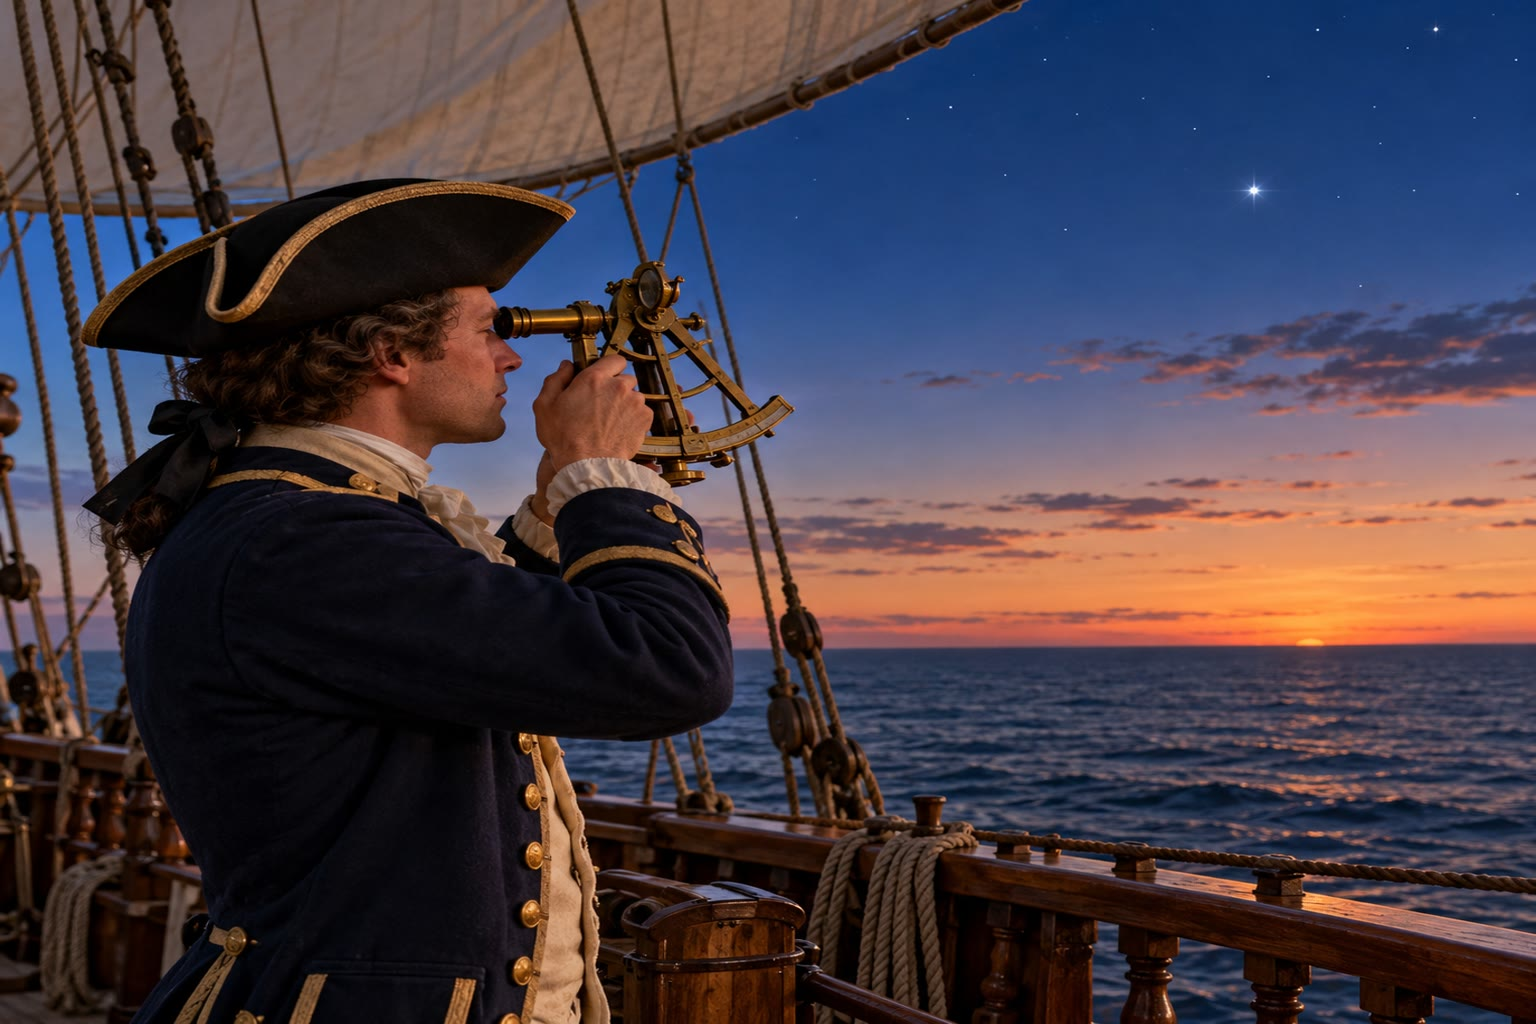
\includegraphics[width=0.62\linewidth]{images/book1/ai/g6-navigator-sextant.jpg}

{\small A navigator of the eighteenth century measures the height of a
star above the \omterm{def:g2:water-on-earth:ocean}{sea} horizon. (AI illustration.)}
\end{omfigure}

\begin{recall}
A \omterm{def:g3:continents-and-oceans:globe}{globe} is a small model of the Earth. The \omterm{def:g3:continents-and-oceans:equator}{equator} is the line that runs
round the middle of the \omterm{def:g3:continents-and-oceans:globe}{globe}, halfway between the \omterm{def:g3:continents-and-oceans:poles}{North Pole} and the \omterm{def:g3:continents-and-oceans:poles}{South
Pole}; it cuts the Earth into the \omterm{def:g3:continents-and-oceans:equator}{northern hemisphere} and the \omterm{def:g3:continents-and-oceans:equator}{southern
hemisphere} (\cref{ch:g3:continents-and-oceans}). The physics books showed
that the Earth turns on itself around an axis through the two \omterm{def:g3:continents-and-oceans:poles}{poles}, once
in a day: this turning brings day and night.
\end{recall}

\section{Parallels and latitude}

To say where a place is on the Earth, we need two numbers, like the row
and the column of a seat in a cinema. The first one tells how far north or
south of the \omterm{def:g3:continents-and-oceans:equator}{equator} the place lies.

Imagine the Earth cut in two, through both \omterm{def:g3:continents-and-oceans:poles}{poles}, like an apple cut from
the stalk downwards. On the cut face (left, below), the \omterm{def:g3:continents-and-oceans:equator}{equator} is the
horizontal line through the centre. A place~P on the surface is seen from
the centre at a certain angle above or below that line: this angle is its
\omterm{def:g6:latitude-longitude:latitude}{latitude}.

\begin{omfigure}
\begin{minipage}[t]{0.48\linewidth}\centering
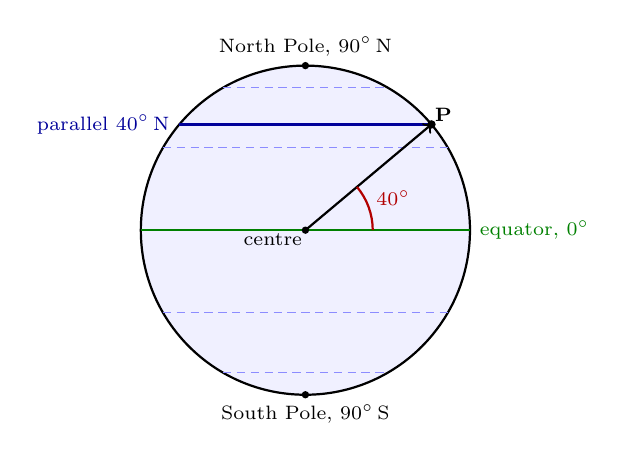
\begin{tikzpicture}[scale=0.95]
  \def\R{2.2}
  \fill[blue!6] (0,0) circle (\R);
  \draw[thick] (0,0) circle (\R);
  % parallels seen edge-on: horizontal chords
  \foreach \a in {-60,-30,30,60}{
    \draw[blue!45, densely dashed] ({-\R*cos(\a)},{\R*sin(\a)}) -- ({\R*cos(\a)},{\R*sin(\a)});}
    \draw[green!50!black, thick] (-\R,0) -- (\R,0);
  \node[font=\scriptsize, green!50!black, anchor=west] at (\R,0) {equator, $0^\circ$};
  \draw[blue!60!black, thick] ({-\R*cos(40)},{\R*sin(40)}) -- ({\R*cos(40)},{\R*sin(40)});
  \draw[->, thick] (0,0) -- ({\R*cos(40)},{\R*sin(40)});
  \fill (0,0) circle (1.4pt) node[below left, font=\scriptsize, inner sep=1pt] {centre};
  \fill ({\R*cos(40)},{\R*sin(40)}) circle (1.6pt)
    node[above right, font=\scriptsize\bfseries, inner sep=1pt] {P};
  \draw[red!70!black, thick] (0.9,0) arc (0:40:0.9);
  \node[red!70!black, font=\scriptsize] at (20:1.25) {$40^\circ$};
  \node[font=\scriptsize, blue!60!black, anchor=east] at ({-\R*cos(40)},{\R*sin(40)}) {parallel $40^\circ$\,N};
  \fill (0,\R) circle (1.4pt) node[above, font=\scriptsize] {North Pole, $90^\circ$\,N};
  \fill (0,-\R) circle (1.4pt) node[below, font=\scriptsize] {South Pole, $90^\circ$\,S};
\end{tikzpicture}

{\small \omterm{def:g6:latitude-longitude:latitude}{Latitude}: the angle at the centre of the Earth between the \omterm{def:g3:continents-and-oceans:equator}{equator}
and the place.}
\end{minipage}\hfill
\begin{minipage}[t]{0.48\linewidth}\centering
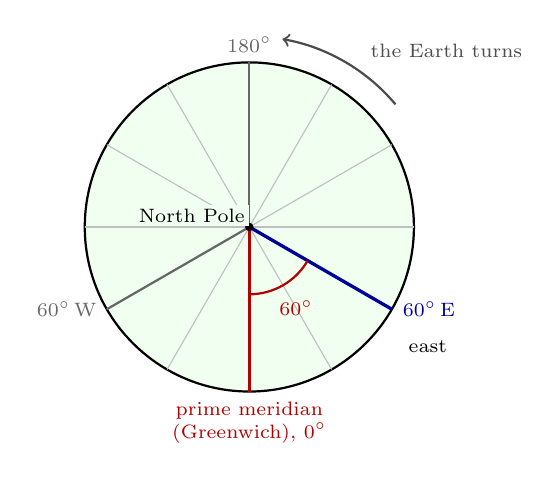
\begin{tikzpicture}[scale=0.95]
  \def\R{2.2}
  \fill[green!6] (0,0) circle (\R);
  \draw[thick] (0,0) circle (\R);
  \foreach \a in {0,30,...,330}{\draw[black!25] (0,0) -- (\a:\R);}
    \draw[red!70!black, very thick] (0,0) -- (270:\R)
    node[below, font=\scriptsize, align=center] {prime meridian\\(Greenwich), $0^\circ$};
  \draw[blue!60!black, very thick] (0,0) -- (330:\R)
    node[right, font=\scriptsize] {$60^\circ$\,E};
  \draw[black!60, thick] (0,0) -- (210:\R) node[left, font=\scriptsize] {$60^\circ$\,W};
  \draw[black!60, thick] (0,0) -- (90:\R) node[above, font=\scriptsize] {$180^\circ$};
  \draw[red!70!black, thick] (270:0.9) arc (270:330:0.9);
  \node[red!70!black, font=\scriptsize] at (300:1.25) {$60^\circ$};
    \fill (0,0) circle (1.6pt) node[above left, font=\scriptsize, inner sep=1.5pt, fill=green!6] {North Pole};
  \draw[->, thick, black!70] (40:2.55) arc (40:80:2.55);
  \node[font=\scriptsize, black!70, anchor=south west] at (55:2.6) {the Earth turns};
  \node[font=\scriptsize, anchor=west] at (2.0,-1.6) {east $\circlearrowleft$};
\end{tikzpicture}

{\small \omterm{def:g6:latitude-longitude:longitude}{Longitude}: the Earth seen from above the \omterm{def:g3:continents-and-oceans:poles}{North Pole}. The angle is
measured from the \omterm{def:g6:latitude-longitude:longitude}{prime meridian}, towards the east or towards the west.}
\end{minipage}
% ledger: rmg:latitude-def, rmg:longitude-def
\end{omfigure}

\begin{definition}[Parallel and latitude]\label{def:g6:latitude-longitude:latitude}
A \emph{parallel}\index{parallel} is a circle drawn round the \omterm{def:g3:continents-and-oceans:globe}{globe} parallel
to the \omterm{def:g3:continents-and-oceans:equator}{equator}; all the places on the same parallel are at the same distance
from the \omterm{def:g3:continents-and-oceans:equator}{equator}. The \emph{latitude}\index{latitude} of a place is the angle,
measured at the centre of the Earth, between the \omterm{def:g3:continents-and-oceans:equator}{equator} and that place. It
goes from $0^\circ$ at the \omterm{def:g3:continents-and-oceans:equator}{equator} to $90^\circ$ at the \omterm{def:g3:continents-and-oceans:poles}{poles}, and we say
whether the place is north (N) or south (S) of the \omterm{def:g3:continents-and-oceans:equator}{equator}.
% ledger: rmg:latitude-def
\end{definition}

The \omterm{def:g3:continents-and-oceans:equator}{equator} is itself a \omterm{def:g6:latitude-longitude:latitude}{parallel}, the longest one, with \omterm{def:g6:latitude-longitude:latitude}{latitude} $0^\circ$.
The \omterm{def:g6:latitude-longitude:latitude}{parallels} get shorter towards the \omterm{def:g3:continents-and-oceans:poles}{poles}, and each \omterm{def:g3:continents-and-oceans:poles}{pole} is a single
point, at $90^\circ$\,N or $90^\circ$\,S. Along a line from a \omterm{def:g3:continents-and-oceans:poles}{pole} to the
\omterm{def:g3:continents-and-oceans:equator}{equator}, each degree of \omterm{def:g6:latitude-longitude:latitude}{latitude} measures about \qty{111}{km}.
% ledger: rmg:latitude-def

\omterm{def:g6:latitude-longitude:latitude}{Latitude} is the easy number: it can be found from the sky. By day,
sailors measured the height of the Sun at noon; at night, in the \omterm{def:g3:continents-and-oceans:equator}{northern
hemisphere}, they measured the height of the Pole Star. That is what the
navigator of the opening picture is doing.
% ledger: rmg:15deg-per-hour

The Pole Star sits almost exactly on the line of the Earth's axis,
prolonged beyond the \omterm{def:g3:continents-and-oceans:poles}{North Pole}, and so far away that its light reaches
every place on the Earth along parallel lines. At the \omterm{def:g3:continents-and-oceans:poles}{North Pole} it is
straight overhead, at $90^\circ$ above the horizon; at the \omterm{def:g3:continents-and-oceans:equator}{equator} it lies
on the northern horizon, at $0^\circ$. In between, the rule is simple:
\emph{the height of the Pole Star above the northern horizon, measured as
an angle, is equal to the \omterm{def:g6:latitude-longitude:latitude}{latitude}}. The figure below shows why the two
angles are the same.
% ledger: nsta:polaris-latitude

\begin{omfigure}
\begin{tikzpicture}[scale=1.1, font=\scriptsize]
  \def\R{1.7}
  \coordinate (O) at (0,0);
  \coordinate (P) at ({\R*cos(40)},{\R*sin(40)});
  \fill[blue!8] (O) circle (\R);
  \draw[black!70] (O) circle (\R);
  % equator and axis
  \draw[black!50] (-\R,0) -- (\R,0);
  \node[black!60, anchor=north east] at (-0.15,0) {equator};
  \draw[black!70, -{Stealth[length=2mm]}] (0,-\R-0.3) -- (0,\R+1.7);
  \node[anchor=east, align=right] at (-0.1,\R+1.45) {towards the Pole Star\\(very far away)};
  \node[anchor=south east] at (0,\R) {N};
  % radius to P and latitude angle at the centre
  \draw[black!80] (O) -- (P);
  \draw[red!70!black, thick] (0.55,0) arc (0:40:0.55);
  \node[red!70!black] at (20:0.8) {$40^\circ$};
  % horizon at P (tangent) and the ray to the Pole Star (parallel to the axis)
  \draw[black!70, thick] ($(P)+({-sin(40)*1.5},{cos(40)*1.5})$) -- ($(P)+({sin(40)*1.6},{-cos(40)*1.6})$);
  \node[anchor=south, rotate=-50, inner sep=2pt] at ($(P)+({sin(40)*1.15},{-cos(40)*1.15})$) {horizon};
  \draw[orange!80!black, thick, -{Stealth[length=2mm]}] (P) -- ++(0,1.45);
  \draw[red!70!black, thick] ($(P)+(0,0.7)$) arc (90:130:0.7);
  \node[red!70!black] at ($(P)+(110:0.98)$) {$40^\circ$};
  \fill (P) circle (1.4pt);
  \node[anchor=west] at ($(P)+(0.3,0.05)$) {observer at $40^\circ$\,N};
\end{tikzpicture}

{\small Why the height of the Pole Star equals the \omterm{def:g6:latitude-longitude:latitude}{latitude} (a sketch, not
to scale). The light of the Pole Star arrives parallel to the Earth's axis
(orange). The horizon of the observer is at right angles to the radius
through the observer; the axis is at right angles to the \omterm{def:g3:continents-and-oceans:equator}{equator}. So the angle
between the horizon and the Pole Star is the same as the \omterm{def:g6:latitude-longitude:latitude}{latitude}, the
angle at the centre between the \omterm{def:g3:continents-and-oceans:equator}{equator} and the observer.}
% ledger: nsta:polaris-latitude
\end{omfigure}

\begin{example}[A navigator at night]\label{ex:g6:latitude-longitude:pole-star}
A navigator measures the Pole Star at $41^\circ$ above the northern
horizon. The ship is at \omterm{def:g6:latitude-longitude:latitude}{latitude} $41^\circ$\,N, about $41 \times 111
\approx \num{4550}$~km north of the \omterm{def:g3:continents-and-oceans:equator}{equator}. Sailing north, she finds the
star a little higher each night; sailing south towards the \omterm{def:g3:continents-and-oceans:equator}{equator}, it
sinks towards the horizon. South of the \omterm{def:g3:continents-and-oceans:equator}{equator} the Pole Star cannot be
seen at all, since it stays below the horizon: there, the noon Sun gives
the \omterm{def:g6:latitude-longitude:latitude}{latitude}.
\end{example}
% ledger: nsta:polaris-latitude, rmg:latitude-def, rmg:15deg-per-hour

\section{Meridians and longitude}

The second number tells how far east or west a place lies. Here there is no
natural starting line like the \omterm{def:g3:continents-and-oceans:equator}{equator}: one has to be chosen.

\begin{definition}[Meridian, longitude and prime meridian]\label{def:g6:latitude-longitude:longitude}
A \emph{meridian}\index{meridian} is a half-circle drawn on the \omterm{def:g3:continents-and-oceans:globe}{globe} from the
\omterm{def:g3:continents-and-oceans:poles}{North Pole} to the \omterm{def:g3:continents-and-oceans:poles}{South Pole}. The \emph{prime meridian}\index{prime meridian}
is the meridian chosen as the starting line: the one that passes through the
old Royal Observatory at Greenwich, in London. The
\emph{longitude}\index{longitude} of a place is the angle between the prime
meridian and the meridian of that place, seen from the axis of the Earth. It
goes from $0^\circ$ at the prime meridian to $180^\circ$, and we say whether
the place is east (E) or west (W) of the prime meridian.
% ledger: rmg:longitude-def
\end{definition}

All the \omterm{def:g6:latitude-longitude:longitude}{meridians} meet at the \omterm{def:g3:continents-and-oceans:poles}{poles}, and they all have the same length. On
the opposite side of the Earth from Greenwich, the \omterm{def:g6:latitude-longitude:longitude}{meridian} $180^\circ$\,E
and the \omterm{def:g6:latitude-longitude:longitude}{meridian} $180^\circ$\,W are the same line.

\begin{omfigure}
\begin{minipage}[c]{0.46\linewidth}\centering
\begin{tikzpicture}
  \begin{axis}[axis equal image, hide axis, width=\linewidth,
      xmin=-1.05, xmax=1.05, ymin=-1.05, ymax=1.12, clip=false]
    \fill[omSea] (axis cs:0,0) circle (1);
    \addplot[fill=omLithAlluv, draw=black!45, line width=0.2pt] table {figdata/out/grade-6-graticule-land.dat};
    \addplot[blue!50!black, line width=0.35pt] table {figdata/out/grade-6-graticule-parallels.dat};
    \addplot[black!55, line width=0.35pt] table {figdata/out/grade-6-graticule-meridians.dat};
        \addplot[green!50!black, line width=1.1pt] table {figdata/out/grade-6-graticule-equator.dat};
    \addplot[red!70!black, line width=1.1pt] table {figdata/out/grade-6-graticule-prime.dat};
    \draw[black!70] (axis cs:0,0) circle (1);
    \fill (axis cs:0,0.9063) circle (1.3pt);
        \node[font=\scriptsize, above left, inner sep=1.5pt] at (axis cs:0,0.9063) {N};
  \end{axis}
\end{tikzpicture}
\end{minipage}\hfill
\begin{minipage}[c]{0.5\linewidth}
{\small A \omterm{def:g3:continents-and-oceans:globe}{globe} with its \omterm{def:g6:latitude-longitude:latitude}{parallels} (blue) and \omterm{def:g6:latitude-longitude:longitude}{meridians} (grey), every
$30^\circ$. The \omterm{def:g3:continents-and-oceans:equator}{equator} is drawn in thick green, the \omterm{def:g6:latitude-longitude:longitude}{prime meridian} in
red; they cross in the \omterm{def:g2:water-on-earth:ocean}{ocean} south of Ghana, at \omterm{def:g6:latitude-longitude:latitude}{latitude} $0^\circ$,
\omterm{def:g6:latitude-longitude:longitude}{longitude} $0^\circ$. Every \omterm{def:g6:latitude-longitude:longitude}{meridian} runs from \omterm{def:g3:continents-and-oceans:poles}{pole} to \omterm{def:g3:continents-and-oceans:poles}{pole}; every \omterm{def:g6:latitude-longitude:latitude}{parallel}
is a circle around the axis. (Land: Natural Earth.)}
% ledger: data:ne-land (figdata/grade-6/graticule.py)
\end{minipage}
\end{omfigure}

\begin{history}[Choosing the prime meridian]
For a long time, each country drew its \omterm{def:g2:drawing-to-map:map}{maps} with its own starting \omterm{def:g6:latitude-longitude:longitude}{meridian}:
London, Paris and other places were all used. In October 1884, delegates of
many countries met in Washington to choose one \omterm{def:g6:latitude-longitude:longitude}{meridian} for the whole world.
On 13~October, they voted to propose the \omterm{def:g6:latitude-longitude:longitude}{meridian} passing through the
observatory of Greenwich: 21 countries voted for it, one against, and two
did not vote.
% ledger: rmg:longitude-def, meridian:1884-vote
\end{history}

\section{Finding a place by its two angles}

With its \omterm{def:g6:latitude-longitude:latitude}{latitude} and its \omterm{def:g6:latitude-longitude:longitude}{longitude}, any place on the Earth can be found,
on a \omterm{def:g2:drawing-to-map:map}{map} or on a \omterm{def:g3:continents-and-oceans:globe}{globe}. We write the \omterm{def:g6:latitude-longitude:latitude}{latitude} first: Cairo, for example, is
at about $30^\circ$\,N, $31^\circ$\,E.
% ledger: data:b1-ne-places (figdata/grade-6/cities.py)

\begin{omfigure}
\begin{tikzpicture}
  \begin{axis}[ommap, width=\linewidth,
      xtick={-180,-150,...,180}, ytick={-90,-60,...,90},
      xticklabels={$180^\circ$,$150^\circ$W,$120^\circ$W,$90^\circ$W,$60^\circ$W,$30^\circ$W,$0^\circ$,
                   $30^\circ$E,$60^\circ$E,$90^\circ$E,$120^\circ$E,$150^\circ$E,$180^\circ$},
      yticklabels={$90^\circ$S,$60^\circ$S,$30^\circ$S,$0^\circ$,$30^\circ$N,$60^\circ$N,$90^\circ$N},
      tick label style={font=\tiny}, grid style={black!35, line width=0.3pt}]
    \addplot[fill=omLithAlluv, draw=black!45, line width=0.2pt] table {figdata/out/shared-geo-land.dat};
        \draw[green!50!black, line width=0.9pt] (axis cs:-180,0) -- (axis cs:180,0);
    \draw[red!70!black, line width=0.9pt] (axis cs:0,-90) -- (axis cs:0,90);
    \addplot[only marks, mark=*, mark size=1.2pt, black,
        point meta=explicit symbolic,
        visualization depends on={value \thisrow{anchor}\as\anc},
        nodes near coords, nodes near coords style={font=\tiny, inner sep=1.2pt,
          anchor=\anc, fill=white, fill opacity=0.75, text opacity=1}]
      table[x=lon, y=lat, meta=name] {figdata/out/grade-6-cities-map.dat};
  \end{axis}
\end{tikzpicture}

{\small Thirteen cities on a \omterm{def:g3:continents-and-oceans:world-map}{world map} with a grid every $30^\circ$. The
\omterm{def:g3:continents-and-oceans:equator}{equator} is drawn in green, the \omterm{def:g6:latitude-longitude:longitude}{prime meridian} in red. (Coastlines and
cities: Natural Earth.)}
% ledger: data:ne-land, data:b1-ne-places (figdata/grade-6/cities.py, part map)
\end{omfigure}

\begin{method}[Locating a place by its coordinates]\label{met:g6:latitude-longitude:locating}
\begin{enumerate}
  \item \omterm{def:g6:latitude-longitude:latitude}{Latitude}: start from the \omterm{def:g3:continents-and-oceans:equator}{equator} and go north (N) or south (S),
        counting the \omterm{def:g6:latitude-longitude:latitude}{parallels}, up to the right number of degrees.
  \item \omterm{def:g6:latitude-longitude:longitude}{Longitude}: start from the \omterm{def:g6:latitude-longitude:longitude}{prime meridian} and go east (E) or west
        (W), counting the \omterm{def:g6:latitude-longitude:longitude}{meridians}, up to the right number of degrees.
  \item The place is where the \omterm{def:g6:latitude-longitude:latitude}{parallel} and the \omterm{def:g6:latitude-longitude:longitude}{meridian} cross. Between two
        lines of the grid, estimate: halfway between $30^\circ$ and
        $60^\circ$ is $45^\circ$.
\end{enumerate}
\end{method}

\begin{example}[Reading the coordinates of Sydney]\label{ex:g6:latitude-longitude:sydney}
On the \omterm{def:g2:drawing-to-map:map}{map}, Sydney lies below the \omterm{def:g3:continents-and-oceans:equator}{equator}: it is in the \omterm{def:g3:continents-and-oceans:equator}{southern
hemisphere}, a little above the \omterm{def:g6:latitude-longitude:latitude}{parallel} $30^\circ$\,S, closer to $30^\circ$
than to $60^\circ$; its \omterm{def:g6:latitude-longitude:latitude}{latitude} is about $34^\circ$\,S. It lies to the right
of the \omterm{def:g6:latitude-longitude:longitude}{prime meridian}, a little beyond the \omterm{def:g6:latitude-longitude:longitude}{meridian} $150^\circ$\,E; its
\omterm{def:g6:latitude-longitude:longitude}{longitude} is about $151^\circ$\,E. We write: Sydney, $34^\circ$\,S,
$151^\circ$\,E.
% ledger: data:b1-ne-places (cities.py: 33.87 S, 151.21 E)
\end{example}

\section{The turning Earth and the time zones}

The Earth turns on itself once a day, from west to east. As it turns, the
Sun seems to cross the sky from east to west. When the Sun is at its highest
in the sky, it is noon. But it is not noon everywhere at the same moment:
when it is noon in London, it is already afternoon in Cairo, further east,
and still morning in New York, further west.

How much does the Earth turn in one hour? A whole turn is $360^\circ$, and
it takes 24~hours:
\[
360^\circ \div 24 = 15^\circ \text{ per hour.}
\]
So two places $15^\circ$ of \omterm{def:g6:latitude-longitude:longitude}{longitude} apart have their noon one hour apart:
the place further east has it first. One degree takes 4~minutes.
% ledger: planet:Earth.day, rmg:15deg-per-hour

\begin{definition}[Time zone]\label{def:g6:latitude-longitude:time-zone}
A \emph{time zone}\index{time zone} is a band of the Earth, from \omterm{def:g3:continents-and-oceans:poles}{pole} to
\omterm{def:g3:continents-and-oceans:poles}{pole}, where all the clocks show the same time. Ideally, each zone is
$15^\circ$ of \omterm{def:g6:latitude-longitude:longitude}{longitude} wide, so that there are 24 zones, one for each
hour; going one zone to the east, the clocks show one hour more.
\end{definition}

In the ideal zones, the zone of a place is its \omterm{def:g6:latitude-longitude:longitude}{longitude} divided by $15$,
rounded to the nearest whole number: east of Greenwich we add that many
hours to the time at Greenwich, west of it we subtract them. Tokyo, at
$140^\circ$\,E: $140 \div 15 \approx 9.3$, so the zone is $+9$: when it is
noon at Greenwich, it is 9~p.m. in Tokyo. Real \omterm{def:g6:latitude-longitude:time-zone}{time zones} are not straight
bands: they follow the borders of countries and regions, so that a whole
country, or a whole region, keeps the same time.
% ledger: data:b1-ne-places, rmg:15deg-per-hour

\begin{omfigure}
\begin{tikzpicture}
  \begin{axis}[ommap, width=\linewidth, clip=false,
      xtick={-180,-90,0,90,180}, ytick={-60,0,60},
      xticklabels={$180^\circ$,$90^\circ$W,$0^\circ$,$90^\circ$E,$180^\circ$},
      yticklabels={$60^\circ$S,$0^\circ$,$60^\circ$N},
      tick label style={font=\tiny}, grid=none]
    \addplot[fill=black!8, draw=none] table {figdata/out/grade-6-time_zones-odd.dat};
    \addplot[fill=omLithAlluv, fill opacity=0.85, draw=black!45, line width=0.2pt] table {figdata/out/shared-geo-land.dat};
    \addplot[only marks, mark=none, point meta=explicit symbolic,
        nodes near coords, nodes near coords style={font=\tiny, anchor=south, inner sep=1pt}]
            table[x=lon, y=y, meta=label] {figdata/out/grade-6-time_zones-labels.dat};
    \draw[red!75!black, line width=1.6pt] (axis cs:180,-90) -- (axis cs:180,90);
    \draw[red!75!black, line width=1.6pt] (axis cs:-180,-90) -- (axis cs:-180,90);
        \draw[black, line width=0.8pt] (axis cs:0,-90) -- (axis cs:0,90);
    \node[font=\scriptsize, red!75!black, rotate=90, anchor=south] at (axis cs:180,0) {date line};
    \node[font=\scriptsize, red!75!black, rotate=90, anchor=north] at (axis cs:-180,0) {date line};
  \end{axis}
\end{tikzpicture}

{\small The 24 ideal \omterm{def:g6:latitude-longitude:time-zone}{time zones}, each $15^\circ$ wide, with the number of
hours to add to the time at Greenwich (the black line in the middle). The date line runs
along the $180^\circ$ \omterm{def:g6:latitude-longitude:longitude}{meridian}, which this \omterm{def:g2:drawing-to-map:map}{map} cuts in two: it is both the
left and the right edge. Roll the \omterm{def:g2:drawing-to-map:map}{map} into a tube, and the two red lines
become one. The zone on each side of the date line is half a zone wide.}
% ledger: rmg:15deg-per-hour, planet:Earth.day (figdata/grade-6/time_zones.py)
\end{omfigure}

\paragraph{The date line.} Travel east from Greenwich, adding one hour per
zone: at $180^\circ$ you are 12~hours ahead. Travel west, subtracting one
hour per zone: at $180^\circ$ you are 12~hours behind. The two travellers
meet on the same \omterm{def:g6:latitude-longitude:longitude}{meridian} with clocks showing the same hour, but a whole day
apart! One of them must change the date.

\begin{definition}[International date line]\label{def:g6:latitude-longitude:date-line}
The \emph{international date line}\index{international date line} is the
line, in the middle of the Pacific \omterm{def:g2:water-on-earth:ocean}{Ocean}, where the date changes. It follows
the $180^\circ$ \omterm{def:g6:latitude-longitude:longitude}{meridian}, with a few bends so as not to cut a country in two.
Crossing it towards the west, we move to the next day; crossing it towards
the east, we go back to the day before.
\end{definition}

\begin{history}[Harrison's sea watch]
\begin{minipage}[c]{0.7\linewidth}
To find his \omterm{def:g6:latitude-longitude:longitude}{longitude}, a navigator compares two times: the local time on
the ship, read from the Sun, and at the same moment the time at a home port.
Each hour of difference means $15^\circ$ of \omterm{def:g6:latitude-longitude:longitude}{longitude}. The difficulty was
to carry the home time across the \omterm{def:g2:water-on-earth:ocean}{ocean}: even the best watches of the time
were not accurate enough. The English clockmaker John Harrison spent decades
on the problem, aiming at a clock that would not gain or lose more than
3~seconds a day. His fourth \omterm{def:g2:water-on-earth:ocean}{sea} timekeeper, called H4, looks like a large pocket
watch and ticks five times a second. In 1761, his son William took it on a
voyage to Jamaica to test it.
% ledger: rmg:15deg-per-hour, rmg:longitude-act-1714, rmg:h4-jamaica-1761
\end{minipage}\hfill
\begin{minipage}[c]{0.26\linewidth}\centering
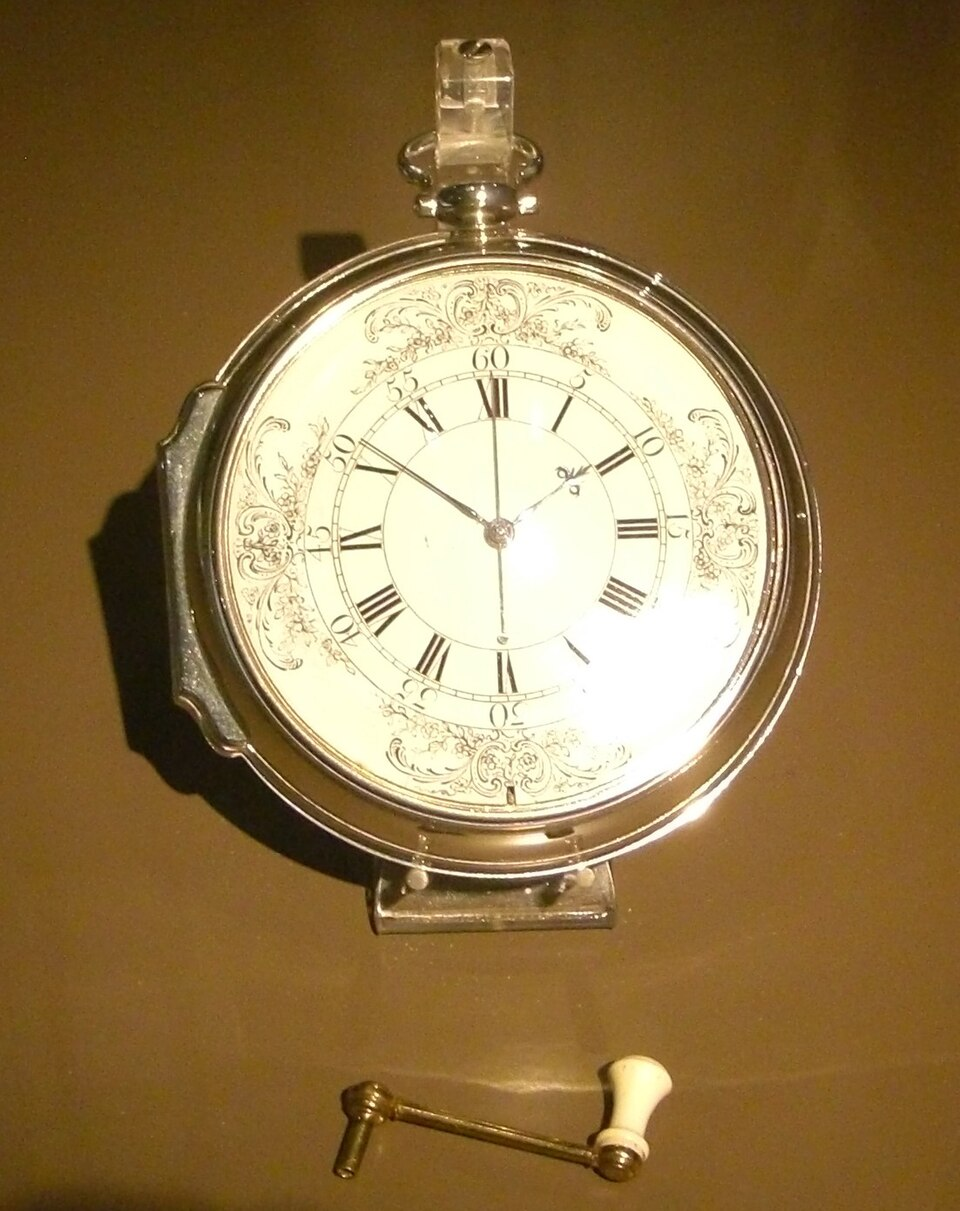
\includegraphics[width=\linewidth]{images/book1/g6-harrison-h4.jpg}\\[2pt]
{\footnotesize Harrison's H4, National Maritime Museum, Greenwich. (Photo:
Colonel Warden, CC BY-SA 3.0, via Wikimedia Commons.)}
% ledger: commons:harrison-h4
\end{minipage}
\end{history}

\section{Exercises}

\begin{exercise}[$\star$]\label{exo:g6:latitude-longitude:1}
Copy and complete: ``\omterm{def:g6:latitude-longitude:latitude}{Latitude} is measured from the \ldots{} and goes from
$0^\circ$ to \ldots; \omterm{def:g6:latitude-longitude:longitude}{longitude} is measured from the \ldots{} \omterm{def:g6:latitude-longitude:longitude}{meridian} and
goes from $0^\circ$ to \ldots''
\end{exercise}

\begin{exercise}[$\star$]\label{exo:g6:latitude-longitude:2}
What is the \omterm{def:g6:latitude-longitude:latitude}{latitude} of the \omterm{def:g3:continents-and-oceans:poles}{North Pole}? Of the \omterm{def:g3:continents-and-oceans:poles}{South Pole}? Of a town on the
\omterm{def:g3:continents-and-oceans:equator}{equator}?
\end{exercise}

\begin{exercise}[$\star$]\label{exo:g6:latitude-longitude:3}
Using the \omterm{def:g2:drawing-to-map:map}{map} of the thirteen cities, say in which \omterm{def:g3:continents-and-oceans:equator}{hemisphere}, northern or
southern, and on which side of the \omterm{def:g6:latitude-longitude:longitude}{prime meridian}, east or west, each of
these cities lies: Sydney, New York, Cairo, Rio de Janeiro.
\end{exercise}

\begin{exercise}[$\star$]\label{exo:g6:latitude-longitude:4}
True or false? Correct the false sentences.
(a) All the \omterm{def:g6:latitude-longitude:longitude}{meridians} meet at the \omterm{def:g3:continents-and-oceans:poles}{poles}.
(b) All the \omterm{def:g6:latitude-longitude:latitude}{parallels} have the same length.
(c) The \omterm{def:g3:continents-and-oceans:equator}{equator} is a \omterm{def:g6:latitude-longitude:latitude}{parallel}.
(d) The \omterm{def:g6:latitude-longitude:longitude}{prime meridian} passes through Paris.
\end{exercise}

\begin{exercise}[$\star\star$]\label{exo:g6:latitude-longitude:5}
Using the \omterm{def:g2:drawing-to-map:map}{map} of the thirteen cities, which city lies at about
$30^\circ$\,N, $31^\circ$\,E? Which one at about $41^\circ$\,N,
$74^\circ$\,W? Give the approximate coordinates of Tokyo.
% ledger: data:b1-ne-places (cities.py main table)
\end{exercise}

\begin{exercise}[$\star\star$]\label{exo:g6:latitude-longitude:6}
Town~A is at \omterm{def:g6:latitude-longitude:longitude}{longitude} $0^\circ$ and town~B at \omterm{def:g6:latitude-longitude:longitude}{longitude} $45^\circ$\,E.
How many hours apart are their noons? In which town is it noon first?
\end{exercise}

\begin{exercise}[$\star\star$]\label{exo:g6:latitude-longitude:7}
Mumbai is at about $73^\circ$\,E. Work out its ideal \omterm{def:g6:latitude-longitude:time-zone}{time zone}. When it is
noon at Greenwich, what time is it in Mumbai, in the ideal zones?
% ledger: data:b1-ne-places (cities.py: 72.88 E, zone +5)
\end{exercise}

\begin{exercise}[$\star\star$]\label{exo:g6:latitude-longitude:8}
Each degree of \omterm{def:g6:latitude-longitude:latitude}{latitude} measures about \qty{111}{km}. How far from the
\omterm{def:g3:continents-and-oceans:equator}{equator} is a town at $30^\circ$\,N, measured along its \omterm{def:g6:latitude-longitude:longitude}{meridian}? How far is
the \omterm{def:g3:continents-and-oceans:poles}{North Pole} from the \omterm{def:g3:continents-and-oceans:equator}{equator}?
% ledger: rmg:latitude-def
\end{exercise}

\begin{exercise}[$\star\star$]\label{exo:g6:latitude-longitude:9}
New York is in the zone $-5$ and Tokyo in the zone $+9$. How many hours
apart are their clocks? When it is 8~a.m. on Monday in New York, what time
and what day is it in Tokyo?
% ledger: data:b1-ne-places (cities.py: zones -5 and +9)
\end{exercise}

\begin{exercise}[$\star\star$]\label{exo:g6:latitude-longitude:10}
Lena says: ``The Sun rises in the east, so the towns in the east see the
Sun rise before the towns in the west.'' Is she right? Explain with the
turning of the Earth.
\end{exercise}

\begin{exercise}[$\star\star\star$]\label{exo:g6:latitude-longitude:11}
A ship's clock gains 3~seconds a day (it runs too fast). (a) How many
seconds fast is it after a voyage of 42~days? (b) The Earth turns one
degree in 4~minutes, that is 240~seconds. What error, in degrees of
\omterm{def:g6:latitude-longitude:longitude}{longitude}, does the clock's error make? (c) At the \omterm{def:g3:continents-and-oceans:equator}{equator}, one degree of
\omterm{def:g6:latitude-longitude:longitude}{longitude} measures about \qty{111}{km}. About how many kilometres is the
navigator wrong, at the \omterm{def:g3:continents-and-oceans:equator}{equator}?
% ledger: rmg:longitude-act-1714, rmg:15deg-per-hour, rmg:latitude-def
\end{exercise}

\begin{exercise}[$\star\star\star$]\label{exo:g6:latitude-longitude:12}
A plane leaves Tokyo (zone $+9$) at 6~p.m. on Monday and flies east across
the Pacific to Los Angeles (zone $-8$). The flight lasts 10~hours. (a) What
time is it at Greenwich when the plane leaves? (b) What time is it at
Greenwich when it lands? (c) What is the local time and the day in Los
Angeles when it lands? Why do travellers say that on this flight ``you land
before you took off''?
\end{exercise}

\section{Problem: A video call around the world}

\begin{problem}[{Weekend problem --- five friends, four time zones and one
date line: what time is it in Auckland when the call starts?}]
\label{pb:g6:latitude-longitude:1}
% ledger: data:b1-ne-places, rmg:15deg-per-hour, planet:Earth.day (cities.py, time_zones.py; test_cities_zones_used_in_the_problem)
Lena lives in London. She wants to organise a video call with four friends
she met on holiday: Ana in Rio de Janeiro, Kenji in Tokyo, Mia in Auckland
and Sam in Los Angeles. In this problem, we use the ideal \omterm{def:g6:latitude-longitude:time-zone}{time zones}.

\begin{center}
\small
\begin{tabular}{lll}
\hline
friend & city & coordinates\\
\hline
Lena & London & $52^\circ$\,N, $0^\circ$\\
Ana & Rio de Janeiro & $23^\circ$\,S, $43^\circ$\,W\\
Kenji & Tokyo & $36^\circ$\,N, $140^\circ$\,E\\
Mia & Auckland & $37^\circ$\,S, $175^\circ$\,E\\
Sam & Los Angeles & $34^\circ$\,N, $118^\circ$\,W\\
\hline
\end{tabular}
\end{center}

\medskip
\noindent\textbf{Part I --- Where the friends live.}
\begin{enumerate}
  \item Which friends live in the \omterm{def:g3:continents-and-oceans:equator}{southern hemisphere}?
  \item Which friends live west of the \omterm{def:g6:latitude-longitude:longitude}{prime meridian}?
  \item Which friend lives farthest from the \omterm{def:g3:continents-and-oceans:equator}{equator}?
  \item Which friend lives closest to the $180^\circ$ \omterm{def:g6:latitude-longitude:longitude}{meridian}? How many
        degrees of \omterm{def:g6:latitude-longitude:longitude}{longitude} away from it?
\end{enumerate}

\medskip
\noindent\textbf{Part II --- What time is it?}
\begin{enumerate}[resume]
  \item How many degrees does the Earth turn in one hour?
  \item Work out the ideal \omterm{def:g6:latitude-longitude:time-zone}{time zone} of each friend's city.
  \item Lena proposes to start the call on Friday at 8~p.m., London time.
        What time and what day is it then in Rio de Janeiro? In Tokyo?
  \item Kenji answers that he will be asleep. Explain why it is already
        Saturday in Tokyo.
\end{enumerate}

\medskip
\noindent\textbf{Part III --- Crossing the date line.}
\begin{enumerate}[resume]
  \item What time and what day is it in Los Angeles when the call starts?
  \item How many hours ahead of Los Angeles are the clocks of Auckland?
  \item Sailing east from Auckland to Los Angeles, a ship crosses the date
        line. Does it go forward to the next day or back to the day before?
  \item What is the local time, and the day, in Auckland when the call
        starts?
\end{enumerate}
\end{problem}
